\chapter{小样本HRRP RATR 技术基本原理}
\label{chap:theory}

\section{引言}
\label{sec:theory_intro}

为了能够针对性地设计和改进元学习方法以适应小样本HRRP识别的特定需求,深刻理解其面临挑战的根源以及所能利用的理论工具至关重要。本章的核心任务正是为此奠定坚实的理论基础。我们将首先深入剖析HRRP的成像机理与数学表达,并着重分析其关键特性,尤其是导致识别困难的噪声影响和角度敏感性问题,为后续算法设计提供物理层面的洞察。接着,我们将回顾基于深度学习的RATR基本框架,明确元学习所依托或改进的现有模型基础。最后,也是本章的重点,我们将对小样本学习问题进行严格的形式化定义,并系统阐述元学习的基本概念、主流范式(基于优化、基于度量)及其核心算法机制,为后续章节中提出的创新元学习解决方案提供必要的算法背景和理论支撑。

本章具体内容安排如下:第\ref{sec:hrrp_mechanism}节介绍HRRP成像模型及特性分析;第\ref{sec:深度学习_ratr}节阐述基于深度学习的RATR技术框架与典型模型;第\ref{sec:fsl_modeling}节对小样本学习与元学习进行形式化定义并介绍基本框架;第\ref{sec:theory_summary}节对本章进行总结。

\section{空天目标宽带雷达成像机理}
\label{sec:hrrp_mechanism}

HRRP的形成是雷达系统发射宽带信号与目标发生电磁相互作用并经接收处理的结果。其精细结构蕴含了目标沿雷达视线(Line of Sight, LOS)方向的散射中心分布信息,是目标识别的重要依据。

\subsection{宽带雷达信号模型与HRRP成像}
\label{subsec:hrrp_imaging_model}

为了获得高的距离分辨率 $\Delta R$,现代雷达通常发射具有大带宽 $B$ 的信号。除了线性调频(Linear Frequency Modulated,LFM)信号,其他宽带信号形式如非线性调频、相位编码信号(如巴克码、P码)、频率步进信号等也可用于高分辨率成像,但LFM因其实现简单、易于产生大时宽带宽积而被广泛使用。一个典型的LFM发射信号 $s_t(t)$ 可以表示为:
\begin{equation}
    s_t(t) = \text{rect}\left(\frac{t}{T_p}\right) A_t \exp\left(j 2\pi f_c t + j \pi \gamma t^2\right)
    \label{eq:lfm_signal}
\end{equation}
其中,$t$ 表示快时间(Fast Time),$T_p$ 是脉冲持续时间,$A_t$ 是发射信号幅度,$f_c$ 是载波中心频率,$\gamma = B / T_p$ 是调频斜率。$\text{rect}(u)$ 是矩形窗函数。信号的瞬时频率为 $f(t) = f_c + \gamma t$,$t \in [-T_p/2, T_p/2]$,覆盖的带宽为 $B = |\gamma| T_p$。

假设目标可以由 $P$ 个理想的点散射中心模型近似描述。设第 $i$ 个散射中心的位置向量为 $\mathbf{r}_i$,其相对于雷达的初始距离为 $R_i = ||\mathbf{r}_i||$,对应的雷达散射系数为 $\sigma_i$(与频率、角度、极化相关)。在远场假设下,并考虑信号传播路径损耗,当雷达发射信号 $s_t(t)$ 后,经过目标散射并在雷达处接收到的回波信号 $s_r(t)$ 可以表示为所有散射中心回波的叠加:
\begin{equation}
    s_r(t) \approx \sum_{i=1}^{P} A_r \frac{\sigma_i}{R_i^2} s_t\left(t - \tau_i(t)\right)
    \label{eq:received_signal_sum_amplitude}
\end{equation}
其中,$A_r$ 是与雷达系统参数(如天线增益、发射功率)相关的幅度因子,$\tau_i(t) = 2 R_i(t) / c$ 是第 $i$ 个散射中心的瞬时双程传播时延,$R_i(t)$ 是 $t$ 时刻该散射中心到雷达的瞬时距离,$c$ 是光速。

在单个脉冲持续时间 $T_p$ 内,对于非机动或慢速目标,通常采用“冻结目标”或“走停”近似。在此近似下,$R_i(t) \approx R_i$。将回波信号下变频到基带,滤除高频项,并补偿固定的路径损耗和系统增益后,基带接收信号 $s_{r,base}(t)$ 近似为:
\begin{equation}
    s_{r,base}(t) \approx \sum_{i=1}^{P} \sigma'_i \text{rect}\left(\frac{t-\tau_i}{T_p}\right) \exp\left(j \pi \gamma (t-\tau_i)^2\right)
    \label{eq:received_baseband}
\end{equation}
其中 $\sigma'_i$ 是包含了幅度、散射相位以及传播相位 $\exp(-j 2\pi f_c \tau_i)$ 的等效复散射系数,$\tau_i = 2R_i/c$。

为了从接收信号中获得高距离分辨率,需要进行脉冲压缩处理,这通常通过与发射信号的复共轭进行匹配滤波来实现。匹配滤波器的冲激响应(基带形式)为 $h(t) = s_t^*(-t) \exp(-j 2\pi f_c t)$。匹配滤波器的输出 $s_o(t)$ 是输入信号与滤波器冲激响应的卷积:
\begin{equation}
    s_o(t) = s_{r,base}(t) * h(t) = \int_{-\infty}^{\infty} s_{r,base}(\tau) h(t-\tau) d\tau
    \label{eq:matched_filtering}
\end{equation}
对于理想的LFM信号和单个点目标,匹配滤波输出近似为一个峰值位于 $t = \tau_1$ 的sinc函数,其幅度包络为 $|\text{sinc}(B(t - \tau_1))|$。对于由多个散射中心组成的目标,在忽略散射中心之间的相互耦合以及满足分辨率要求的前提下,匹配滤波的输出近似为各个散射中心响应的相干叠加:
\begin{equation}
    s_o(t) \approx \sum_{i=1}^{P} \sigma''_i \text{sinc}\left(B(t - \tau_i)\right) \exp(-j 2\pi f_c \tau_i)
    \label{eq:pulse_compression_output_phase}
\end{equation}
其中 $\sigma''_i$ 是包含了原始散射幅度、脉冲压缩增益等因素的复幅度系数。此处的相位项 $\exp(-j 2\pi f_c \tau_i)$ 非常重要,它导致了不同散射中心响应之间的相干干涉。

HRRP通常定义为脉冲压缩后输出信号的幅度(或功率)沿距离轴的分布。令距离 $r = ct/2$,则HRRP函数 $p(r)$ 可以表示为:
\begin{equation}
    p(r) = |s_o(t)|_{t=2r/c} \approx \left| \sum_{i=1}^{P} \sigma''_i \text{sinc}\left(\frac{2B}{c}(r - R_i)\right) \exp(-j \frac{4\pi f_c R_i}{c}) \right|
    \label{eq:hrrp_definition_complex}
\end{equation}
其中 $R_i = c\tau_i/2$ 是第 $i$ 个散射中心沿雷达视线的投影距离。该式更清晰地表明,HRRP是目标各散射中心响应(具有幅度和相位)在距离轴上相干叠加后的幅度包络。其能够分辨两个散射中心的最小距离间隔,即距离分辨率 $\Delta R$,由信号带宽 $B$ 决定:
\begin{equation}
    \Delta R = \frac{\kappa c}{2B}
    \label{eq:range_resolution_kappa}
\end{equation}
其中 $\kappa$ 是与窗函数和分辨率定义相关的因子,对于矩形窗和瑞利准则(主瓣峰值到第一零点),$\kappa \approx 1$。实际应用中,为抑制旁瓣,常使用非矩形窗函数(如汉宁窗、海明窗),这会略微展宽主瓣,即 $\kappa > 1$。

然而,式~(\ref{eq:hrrp_definition_complex})描述的是理想情况下的HRRP。在实际雷达系统中,接收到的信号总是伴随着噪声和杂波。设 $n(t)$ 表示基带接收机噪声,通常建模为零均值加性高斯白噪声(Additive White Gaussian Noise, AWGN),其功率谱密度为 $N_0$。设 $c(t)$ 表示来自环境背景(地面、海面、云雨等)的杂波回波。则实际接收到的基带信号应为:
\begin{equation}
    s_{r,base}^{noisy}(t) = s_{r,base}(t) + c(t) + n(t)
    \label{eq:received_noisy}
\end{equation}
经过匹配滤波后,输出信号变为:
\begin{equation}
    s_o^{noisy}(t) = s_o(t) + c_o(t) + n_o(t)
    \label{eq:output_noisy}
\end{equation}
其中$s_o(t)$是理想目标回波的脉压输出,$c_o(t) = c(t) * h(t)$ 是杂波的脉压输出,$n_o(t) = n(t) * h(t)$ 是噪声的脉压输出。如果 $n(t)$ 是AWGN,则 $n_o(t)$ 也是零均值高斯过程,但不再是白噪声,其自相关函数由 $h(t)$ 决定。杂波 $c(t)$ 的统计特性通常更复杂,可能是非高斯的、相关的,并且其强度随距离、角度、环境类型(如不同地貌、海况)变化,常用的模型有瑞利分布(大量独立小散射体)、韦伯分布、对数正态分布或K分布(用于描述海杂波或地杂波的拖尾现象)\upcite{Jakeman1976806, Marier1995568, Ward1981561, Ozturk1995106}。

因此,实际观测到的HRRP样本 $p^{noisy}(r)$ 是含有噪声和杂波的脉压输出的幅度:
\begin{equation}
    p^{noisy}(r) = |s_o^{noisy}(t)|_{t=2r/c} = |s_o(t) + c_o(t) + n_o(t)|_{t=2r/c}
    \label{eq:hrrp_noisy}
\end{equation}
噪声和杂波的存在会污染甚至淹没目标信号 $s_o(t)$,导致HRRP形态失真、细节丢失、出现虚假峰值,从而严重影响识别性能。SNR或信杂比(Signal-to-Clutter Ratio, SCR)是衡量信号质量的重要指标。例如,脉压后的峰值信噪比可以定义为 $\text{SNR}_{peak} = \max |s_o(t)|^2 / E[|n_o(t)|^2]$。低SNR/SCR是RATR(特别是小样本RATR)面临的第一个严峻问题。虽然杂波(对应SCR)在特定环境(如地面、海面)下是主要的干扰源,其统计特性也更为复杂,但噪声(尤其是接收机热噪声,对应SNR)是雷达系统固有且普遍存在的干扰形式。AWGN模型因其数学上的易处理性和在算法性能评估中的基准地位,被广泛用于模拟和分析噪声对系统性能的影响。因此,本论文在后续章节研究算法的鲁棒性时,将主要聚焦于SNR条件下的性能,并主要采用AWGN模型来模拟噪声干扰,以此作为评估和提升算法在基础噪声环境下稳健性的关键途径,尽管对复杂杂波的抑制亦是重要的研究方向。 后续章节需要研究的算法应具备在低SNR下(即面对式~(\ref{eq:received_noisy})形式的输入时,其中噪声$n(t)$占主导地位)的鲁棒性。


现在我们来更形式化地描述HRRP的角度敏感性问题。如前所述,HRRP的形态依赖于目标姿态角 $(\theta, \phi)$。我们可以将理想HRRP函数显式地写为 $p(r; \theta, \phi)$,或者对于离散HRRP向量,记为 $\mathbf{p}(\theta, \phi) \in \mathbb{R}^N$。根据式~(\ref{eq:hrrp_definition_complex}),这种依赖性主要来源于投影距离 $R_i(\theta, \phi) = \mathbf{r}_i \cdot \hat{\mathbf{k}}(\theta, \phi)$ 和复幅度 $\sigma''_i(\theta, \phi)$ 对视线向量 $\hat{\mathbf{k}}(\theta, \phi)$ 的依赖。当姿态角发生一个微小的变化 $(\Delta\theta, \Delta\phi)$ 时,视线向量变化 $\Delta\hat{\mathbf{k}}$,导致投影距离变化 $\Delta R_i = \mathbf{r}_i \cdot \Delta\hat{\mathbf{k}}$,幅度 $\sigma''_i$ 也会发生变化 $\Delta\sigma''_i$。由于HRRP是相干叠加的结果,即使 $\Delta R_i$ 很小(小于 $\Delta R$),但其引起的相位变化 $\Delta\psi_i = - \frac{4\pi f_c}{c} \Delta R_i$ 可能很大(因 $f_c \gg B$),导致不同散射中心响应的干涉状态(相长或相消)发生剧烈改变,从而引起HRRP幅度 $p(r; \theta, \phi)$ 的快速振荡。我们可以用HRRP向量之间的距离(如欧氏距离)来衡量角度敏感性。对于同一目标 $y$,其在两个不同姿态角 $(\theta_1, \phi_1)$ 和 $(\theta_2, \phi_2)$ 下的HRRP样本 $\mathbf{p}_1 = \mathbf{p}(\theta_1, \phi_1)$ 和 $\mathbf{p}_2 = \mathbf{p}(\theta_2, \phi_2)$ 之间的距离 $d(\mathbf{p}_1, \mathbf{p}_2)$ 可能非常大,即使角度差 $\sqrt{(\theta_1-\theta_2)^2 + (\phi_1-\phi_2)^2}$ 很小。同时,可能存在另一个不同目标 $y'$ 在某个姿态角 $(\theta_3, \phi_3)$ 下的HRRP样本 $\mathbf{p}_3$ 与 $\mathbf{p}_1$ 非常接近,即 $d(\mathbf{p}_1, \mathbf{p}_3)$ 很小。这种现象即 $d(\mathbf{p}_1, \mathbf{p}_2) \gg d(\mathbf{p}_1, \mathbf{p}_3)$,其中 $y_1=y_2=y, y_3=y', y \neq y'$,严重违反了许多模式识别算法所依赖的“类内距离小、类间距离大”的假设。这就是HRRP角度敏感性对识别带来的核心困难,也是小样本RATR面临的第二个关键问题。后续章节需要设计的算法必须能够处理或减轻这种极端角度敏感性的影响。

\subsection{典型空天目标电磁散射特性}
\label{subsec:scattering_characteristics}

理解空天目标的电磁散射特性是深入分析HRRP数据并设计有效识别算法的基础。目标的散射特性决定了雷达接收到的回波信号的强度、相位、极化等信息,从而决定了HRRP的形态。

目标的雷达散射截面积(Radar Cross Section,RCS),记为 $\sigma$,是定量描述目标在特定方向上散射雷达波能力强弱的关键物理量。其严格定义为:
\begin{equation}
    \sigma = \lim_{R \to \infty} 4\pi R^2 \frac{P_s}{P_i} = \lim_{R \to \infty} 4\pi R^2 \frac{|\mathbf{E}_s|^2}{|\mathbf{E}_i|^2}
    \label{eq:rcs_definition}
\end{equation}
其中,$R$ 是距离,$P_i$ 和 $P_s$ 分别是入射和散射功率密度,$\mathbf{E}_i$ 和 $\mathbf{E}_s$ 分别是入射和散射电场强度。RCS具有面积的量纲,单位通常是平方米(m²)或分贝平方米(dBsm)。对于一个复杂目标,RCS不仅依赖于目标的物理属性(尺寸、形状、材料),还强烈地依赖于雷达的工作参数(频率 $f_c$、极化方式 $\text{pol}$)和观测几何(入射波方向 $(\theta_i, \phi_i)$ 和散射波方向 $(\theta_s, \phi_s)$)。对于单站雷达,入射和散射方向相同,RCS通常表示为 $\sigma(f_c, \text{pol}, \theta, \phi)$,其中 $(\theta, \phi)$ 是目标本体坐标系下的姿态角。

根据电磁场理论,在高频区(目标尺寸远大于波长 $\lambda = c/f_c$),目标的总散射场可以看作是由目标表面感应电流和感应磁流辐射产生的场,其贡献主要来自于局部区域,可以分解为几种基本的散射机制\upcite{Pathak199244, Song19971488, KELLER1962116, Ling1989194, Kouyoumjian19741448}。镜面反射发生在尺寸远大于波长的光滑曲面上,满足几何光学反射定律,散射能量集中在镜面反射方向,通常形成RCS方向图中的强峰值。边缘绕射发生在目标几何形状的突变处,如机翼、尾翼的边缘,舵面、舱门的缝隙边缘等。根据几何绕射理论(Geometrical Theory of Diffraction,GTD),边缘绕射的能量相对较弱,但方向性比镜面反射弱,可在更宽的角度范围内观测到\upcite{kohama_gtd_2011}。尖顶或角点绕射发生在目标的尖顶(如机头、导弹弹头)或角点处。爬行波是电磁波入射到目标光滑曲面的阴影边界时,激发沿表面传播的波,并在目标的背向区域再次辐射,对低频散射和阴影区散射有重要贡献。行波是在细长结构(如机翼前缘、天线臂)上,入射波可能激发沿结构传播的波,并在端点或不连续处产生辐射。腔体散射对于具有开放式腔体结构的目标(如飞机的发动机进气道、尾喷口,座舱等)非常重要,入射电磁波会进入腔体内部,经过多次反射和模式转换后再辐射出来,可能形成非常强的散射,并且其散射特性对频率和观测角度通常极为敏感\upcite{anastassiu_review_2003}。一个复杂空天目标(如飞机)的RCS随姿态角的变化曲线通常呈现出极其复杂的起伏形态,峰谷差异可达数十dB,并且在很小的角度间隔内就可能发生剧烈变化\upcite{xu_rcs_1991}。这是因为随着姿态角的改变,雷达视线照射到目标的不同部位,主导的散射机制会发生转换,同时来自不同散射中心的贡献之间的相干干涉关系也会随之改变,导致总散射场的强度发生快速振荡。

为了在高频区对目标的散射特性进行建模和分析,散射中心模型被广泛应用\upcite{liu_scnet_2024, Gerry19991179, Potter19951058, KELLER1962116, Hurst1987986}。该模型将目标的总散射场近似为来自目标上有限个离散的等效散射中心的贡献的相干叠加。属性散射中心模型(Attributed Scattering Center Model,ASCM)是其中一种常用模型\upcite{Potter199779},它不仅给出了散射中心的位置,还描述了其散射强度随频率和角度变化的特性。根据ASCM,第 $i$ 个散射中心对总散射场 $E_s$ 的贡献 $E_i$ 可以表示为频率 $f$ 和视线向量 $\hat{\mathbf{k}}$ 的函数:
\begin{equation}
    E_i(f, \hat{\mathbf{k}}) \approx A_i(\text{pol}) \left(\frac{j f}{f_{ref}}\right)^{\alpha_i} \mathcal{S}_i(f, \hat{\mathbf{k}}) \exp\left(-j \frac{4\pi f}{c} \mathbf{r}_i \cdot \hat{\mathbf{k}}\right)
    \label{eq:ascm}
\end{equation}
在此式中,$A_i(\text{pol})$ 是第 $i$ 个散射中心在参考频率 $f_{ref}$ 和特定极化下的复幅度。$\alpha_i$ 是频率依赖因子,描述了散射幅度随频率的变化关系,其取值与散射机制类型有关(例如,$\alpha_i=1$ 对应镜面反射,$\alpha_i=0$ 对应边缘绕射)。$\mathcal{S}_i(f, \hat{\mathbf{k}})$ 是角度依赖因子,描述散射强度随观测角度的变化。对于局部化散射中心,$\mathcal{S}_i \approx 1$;对于分布式散射中心(如长直边缘),$\mathcal{S}_i$ 可能具有 $\text{sinc}$ 函数形式。$\mathbf{r}_i$ 是第 $i$ 个散射中心的位置向量。$\exp(-j \frac{4\pi f}{c} \mathbf{r}_i \cdot \hat{\mathbf{k}})$ 是由位置决定的相位项,其中 $\mathbf{r}_i \cdot \hat{\mathbf{k}} = R_i$ 即为该散射中心沿视线的投影距离。将式~(\ref{eq:ascm})代入宽带回波模型并进行脉冲压缩,即可得到基于散射中心模型的HRRP表达式。可以看出,HRRP的形态直接由各散射中心的位置 $\mathbf{r}_i$、类型 $\alpha_i$、强度 $A_i$ 以及它们随频率 $f$ 和视线 $\hat{\mathbf{k}}$ 的变化规律 $\mathcal{S}_i$ 共同决定。当姿态角 $(\theta, \phi)$ 变化时,$\hat{\mathbf{k}}$ 改变,导致相位项中的投影距离 $R_i$、角度依赖因子 $\mathcal{S}_i$ 以及可能的幅度 $A_i$ 都发生变化,进而造成HRRP形态的剧烈改变。这进一步从物理模型层面印证了HRRP的角度敏感性。

需要指出的是,除了HRRP所反映的目标沿雷达视线的静态散射结构信息外,目标的部件级运动(即微动),例如飞机涡轮发动机叶片的旋转、直升机旋翼的转动、导弹弹体的进动或章动等,也会在雷达回波中引入除主体平动多普勒之外的附加频率调制,产生微多普勒效应\upcite{gurbuz_data-driven_2018}。这些微多普勒特征蕴含了关于目标内部结构和运行状态的独特动态信息,是目标识别的另一类重要信息来源,尤其对于区分外形相似但内部运动部件不同的目标具有关键作用。然而,微多普勒特征的提取与分析通常依赖于时频分析技术\upcite{yu_local_2019, huang_parameterized_2021, chithra_comprehensive_2023},这与本研究关注的、主要基于脉冲压缩后HRRP幅度信息的识别方法在信号处理层面和特征维度上均有显著不同。鉴于本论文聚焦于解决小样本条件下HRRP识别所面临的噪声鲁棒性与角度敏感性等核心挑战,对微多普勒特征的深入研究与利用将不作为本文探讨的重点,后续章节将集中讨论基于HRRP本身及其衍生特征的识别方法。

综上所述,空天目标复杂的几何结构和材料构成导致了其独特的电磁散射特性,这种特性对频率和观测角度高度敏感,是形成复杂多变HRRP数据的物理根源。深刻理解这些散射机理和特性,对于后续章节中设计能够适应HRRP数据复杂性(特别是角度敏感性)和环境干扰(如噪声)的鲁棒识别算法至关重要。

\section{基于深度学习的RATR技术}
\label{sec:深度学习_ratr}

近年来,深度学习凭借其强大的特征学习和非线性建模能力,已成为推动RATR技术发展的主要动力。基于深度学习的RATR方法旨在通过构建深度神经网络模型,自动从雷达数据中学习具有判别力的特征表示,实现端到端的识别。

\subsection{RATR 的深度学习框架}
\label{subsec:深度学习_framework}

基于深度学习的RATR系统通常遵循一个标准的监督学习框架。假设拥有训练数据集 $D_{train} = \{(\mathbf{x}_i, y_i)\}_{i=1}^{M}$,其中 $\mathbf{x}_i \in \mathcal{X}$ 是雷达观测数据(如HRRP向量 $\mathbf{p}_i \in \mathbb{R}^N$),$y_i \in \mathcal{Y} = \{1, \dots, C\}$ 是对应的目标类别标签。目标是学习一个映射函数 $f_\Theta: \mathcal{X} \rightarrow \mathcal{Y}$,该函数由参数 $\Theta$ 控制,能对未知样本 $\mathbf{x}$ 预测其类别 $\hat{y} = f_\Theta(\mathbf{x})$。

在深度学习框架下,$f_\Theta$ 通常由一个深度神经网络(Deep Neural Network,DNN)实现,可视为复合函数,由多个层组成,每层对其输入进行线性变换和非线性激活。一个包含 $L$ 层的前馈神经网络可表示为:
\begin{align}
    \mathbf{a}^{(l)} &= W^{(l)} \mathbf{h}^{(l-1)} + \mathbf{b}^{(l)} \label{eq:dnn_linear} \\
    \mathbf{h}^{(l)} &= \sigma^{(l)}(\mathbf{a}^{(l)}) \label{eq:dnn_activation}
\end{align}
其中,$l=1, \dots, L$ 是层索引,$\mathbf{h}^{(l)} \in \mathbb{R}^{d_l}$ 是第 $l$ 层的输出,$\mathbf{h}^{(0)} = \mathbf{x}$ 是输入。$W^{(l)} \in \mathbb{R}^{d_l \times d_{l-1}}$ 和 $\mathbf{b}^{(l)} \in \mathbb{R}^{d_l}$ 是权重和偏置。$\sigma^{(l)}(\cdot)$ 是非线性激活函数(如ReLU)。整个网络的参数为 $\Theta = \{W^{(l)}, \mathbf{b}^{(l)}\}_{l=1}^{L}$。

对于 $C$ 类分类任务,最后一层输出 $C$ 维的 logits $\mathbf{z} = \mathbf{a}^{(L)}$。通过 Softmax 函数将 logits 转换为概率分布 $\mathbf{p}(\mathbf{x}) = [p(y=1|\mathbf{x}), \dots, p(y=C|\mathbf{x})]^T$:
\begin{equation}
    p(y=c|\mathbf{x}; \Theta) = \frac{\exp(z_c)}{\sum_{c'=1}^{C} \exp(z_{c'})}, \quad c=1, \dots, C
    \label{eq:softmax}
\end{equation}
最终预测标签 $\hat{y}$ 选择概率最高的类别:
\begin{equation}
    \hat{y} = f_\Theta(\mathbf{x}) = \arg\max_{c \in \{1, \dots, C\}} p(y=c|\mathbf{x}; \Theta)
    \label{eq:prediction}
\end{equation}

模型训练的目标是找到最优参数 $\Theta^*$,使模型在训练数据 $D_{train}$ 上的预测尽可能准确,并具有良好的泛化能力。这通过最小化损失函数 $\mathcal{L}$ 实现。常用的是交叉熵损失:
\begin{equation}
    \mathcal{L}_{CE}(f_\Theta(\mathbf{x}_i), y_i) = -\sum_{c=1}^{C} \mathbb{I}(y_i=c) \log p(y=c|\mathbf{x}_i; \Theta) = -\log p(y=y_i|\mathbf{x}_i; \Theta)
    \label{eq:cross_entropy_loss}
\end{equation}
其中 $\mathbb{I}(\cdot)$ 是指示函数。训练目标是最小化训练集上的平均损失,通常加入正则化项 $\Omega(\Theta)$ 防止过拟合:
\begin{equation}
    \Theta^* = \arg\min_{\Theta} \left\{ \frac{1}{M} \sum_{i=1}^{M} \mathcal{L}_{CE}(f_\Theta(\mathbf{x}_i), y_i) + \lambda \Omega(\Theta) \right\}
    \label{eq:optimization_objective}
\end{equation}
其中 $\lambda \ge 0$ 是正则化系数。此优化问题通常采用基于梯度的迭代算法求解,如随机梯度下降(Stochastic Gradient Descent,SGD)及其变种\upcite{Bottou2018223, LeCun19982278}。利用反向传播算法计算梯度 $\nabla_\Theta \mathcal{L}$,并更新参数:
\begin{equation}
    \Theta_{t+1} \leftarrow \Theta_t - \eta_t \nabla_\Theta \mathcal{L}(\Theta_t; D_{batch})
    \label{eq:sgd_update}
\end{equation}
其中 $\eta_t$ 是学习率。

% --- 示意图占位符 ---
\begin{figure}[h!]
    \centering
    % \includegraphics[width=0.9\linewidth]{figures/深度学习_framework.pdf}
    \fbox{图 2.1: 基于深度学习的RATR框架示意图 (占位符)}
    \caption{展示一个典型的基于深度学习的RATR系统框架,包括输入雷达数据、深度神经网络、输出类别概率以及训练过程。}
    \label{fig:深度学习_framework}
\end{figure}

\subsection{典型深度学习模型及其适用性}
\label{subsec:typical_深度学习_models}

立足于前述基于深度学习的RATR通用框架,针对HRRP数据独特的物理属性与表征形式,研究界已发展并应用了多种特定的深度神经网络架构。HRRP作为目标一维散射信息的载体,其数据形态呈现为一维序列 $\mathbf{p} \in \mathbb{R}^N$($N$为距离单元数),蕴含着丰富的局部结构信息(如散射中心的位置、强度、形状),同时也表现出对观测角度和噪声的高度敏感性。这些特性共同决定了并非所有深度学习模型都同样适用于HRRP识别任务,模型的选择与设计必须充分考虑如何有效提取HRRP中的判别性信息,同时抑制敏感性带来的负面影响。因此,研究人员已成功探索并适配了包括CNN、RNN、LSTM、Transformer以及自编码器(Atuo-Encoder,AE)等多种深度模型,它们各自凭借不同的结构优势,在HRRP特征学习与识别任务中展现出独特的适用性与潜力。

一维卷积神经网络(1D-CNN)因其在提取局部空间(或时间)模式方面的强大能力,并具有一定的平移不变性,被广泛应用于处理HRRP这类一维序列数据\upcite{song_radar_2019, guo_radar_2019}。对于输入HRRP向量 $\mathbf{p} \in \mathbb{R}^{N \times C_{in}}$(这里假设输入可以有 $C_{in}$ 个通道,例如原始幅度、相位或不同预处理结果;若仅为幅度,则 $C_{in}=1$),一个1D-CNN层包含 $C_{out}$ 个卷积核(Filter)。第 $j$ ($j=1, \dots, C_{out}$) 个卷积核 $\mathbf{K}_j \in \mathbb{R}^{F \times C_{in}}$($F$ 为核尺寸)在输入序列上以步长 $S$ 滑动,并考虑填充 $P$(Padding)。输出特征图 $\mathbf{H}_j \in \mathbb{R}^{N'}$ 的第 $n$ 个元素通过以下卷积操作计算得到:
\begin{equation}
    H_{j,n} = \sigma\left( \sum_{c=1}^{C_{in}} \sum_{f=1}^{F} K_{j,f,c} \, p_{n \cdot S + f - P', c} + b_j \right)
    \label{eq:1d_cnn_conv_detailed}
\end{equation}
其中,$p_{n',c}$ 是输入序列在位置 $n'$、通道 $c$ 的值(经过填充处理),$K_{j,f,c}$ 是第 $j$ 个核在位置 $f$、输入通道 $c$ 的权重,$b_j$ 是第 $j$ 个核对应的偏置,$P'$ 与填充 $P$ 和核中心有关,$\sigma(\cdot)$ 是非线性激活函数(如ReLU, LeakyReLU)。输出特征图的长度 $N' = \lfloor (N + 2P - F) / S \rfloor + 1$。通过堆叠多个卷积层(使用不同的核尺寸、步长、填充和通道数,或引入空洞卷积以增大感受野而不增加参数),模型能够学习到HRRP中从低级的边缘、纹理模式到高级的散射中心组合结构的层次化特征表示。

在卷积层之间或之后,通常会插入池化层(Pooling Layer),如最大池化(Max Pooling)或平均池化(Average Pooling)。池化操作在一个局部窗口(大小为 $F_p$,步长为 $\mathcal{S}_p$)内对特征图进行下采样。例如,最大池化输出为:
\begin{equation}
    H'_{j,n} = \max_{i=(n-1)\mathcal{S}_p+1}^{\min(n\mathcal{S}_p, N')} H_{j,i}
    \label{eq:max_pooling}
\end{equation}
池化层的主要作用是降低特征图的空间维度(长度),减少计算量和参数数量,并提供一定程度的局部平移不变性,增强模型对HRRP轻微平移或形变的鲁棒性。

为了构建更深、更有效的CNN模型,研究者引入了先进的网络结构。残差网络 (Residual Network,ResNet)\upcite{resnet} 通过引入“跳跃连接”(Skip Connection)来缓解深度网络训练中的梯度消失问题。其核心思想是学习残差映射 $\mathcal{F}(\mathbf{h}^{(l-1)})$,并将输入 $\mathbf{h}^{(l-1)}$ 直接加到输出上:
\begin{equation}
    \mathbf{h}^{(l)} = \sigma(\mathcal{F}(\mathbf{h}^{(l-1)}; \mathbf{W}^{(l)}) + \mathbf{h}^{(l-1)})
    \label{eq:resnet_block}
\end{equation}
这种恒等映射的捷径使得梯度能够更容易地反向传播到浅层。密集连接网络 (Densely Connected Convolutional Network,DenseNet)\upcite{huang_2017_cvpr} 则更进一步,将每一层与其后所有层直接连接,每一层的输入包含了前面所有层的特征图的拼接:
\begin{equation}
    \mathbf{h}^{(l)} = \sigma(\mathbf{W}^{(l)} [\mathbf{h}^{(0)}, \mathbf{h}^{(1)}, \dots, \mathbf{h}^{(l-1)}] + \mathbf{b}^{(l)})
    \label{eq:densenet_block}
\end{equation}
其中 $[\cdot]$ 表示特征图在通道维度上的拼接。DenseNet通过最大化信息流和特征重用,可以用更少的参数达到很高的性能。这些结构都可以适配到1D-CNN中,用于构建更强大的HRRP特征提取器。1D-CNN因其对局部结构信息的强大捕捉能力,特别适合提取HRRP中由散射中心及其相对位置关系所决定的特征。

RNN及其变种特别适合处理具有时序或序列依赖性的数据。当HRRP数据以随时间 $t$ 或角度 $\alpha$ 变化的序列 $\mathbf{P} = (\mathbf{p}_1, \mathbf{p}_2, \dots, \mathbf{p}_T)$ 形式给出时($\mathbf{p}_t \in \mathbb{R}^N$),RNN能够通过其内部的循环结构来建模序列中的动态信息。标准的RNN在时刻 $t$ 计算隐藏状态 $\mathbf{h}_t \in \mathbb{R}^{d_h}$,该状态依赖于当前输入 $\mathbf{p}_t \in \mathbb{R}^N$ 和前一时刻的隐藏状态 $\mathbf{h}_{t-1}$:
\begin{equation}
    \mathbf{h}_t = \sigma_h(\mathbf{W}_{hh} \mathbf{h}_{t-1} + \mathbf{W}_{xh} \mathbf{p}_t + \mathbf{b}_h)
    \label{eq:rnn_recurrence_dim}
\end{equation}
其中 $\mathbf{W}_{hh} \in \mathbb{R}^{d_h \times d_h}$ 和 $\mathbf{W}_{xh} \in \mathbb{R}^{d_h \times N}$ 是权重矩阵,$\mathbf{b}_h$ 是偏置,$\sigma_h$ 是激活函数。隐藏状态 $\mathbf{h}_t$ 理论上编码了从序列开始到时刻 $t$ 的所有信息。最终的序列表示(如 $\mathbf{h}_T$ 或所有隐藏状态的某种聚合)被用于分类。然而,标准RNN在处理长序列时会遇到梯度消失或爆炸的问题,难以学习长距离依赖关系\upcite{pan_radar_2022}。

LSTM\upcite{tu_novel_2019, jithesh_lstm_2017}通过引入精巧的门控机制(遗忘门 $\mathbf{f}_t$、输入门 $\mathbf{i}_t$、输出门 $\mathbf{o}_t$)和一个独立的细胞状态 $\mathbf{C}_t \in \mathbb{R}^{d_h}$ 来克服这一问题。这些门控制着信息的流入、流出以及在细胞状态中的长期保存。其更新过程如下(输入为 $[\mathbf{h}_{t-1}, \mathbf{p}_t] \in \mathbb{R}^{d_h+N}$):
\begin{align}
    \mathbf{f}_t &= \sigma_g(\mathbf{W}_f [\mathbf{h}_{t-1}, \mathbf{p}_t] + \mathbf{b}_f) \in \mathbb{R}^{d_h} \label{eq:lstm_f_dim} \\
    \mathbf{i}_t &= \sigma_g(\mathbf{W}_i [\mathbf{h}_{t-1}, \mathbf{p}_t] + \mathbf{b}_i) \in \mathbb{R}^{d_h} \label{eq:lstm_i_dim} \\
    \tilde{\mathbf{C}}_t &= \sigma_c(\mathbf{W}_C [\mathbf{h}_{t-1}, \mathbf{p}_t] + \mathbf{b}_C) \in \mathbb{R}^{d_h} \label{eq:lstm_c_tilde_dim} \\
    \mathbf{C}_t &= \mathbf{f}_t \odot \mathbf{C}_{t-1} + \mathbf{i}_t \odot \tilde{\mathbf{C}}_t \in \mathbb{R}^{d_h} \label{eq:lstm_c_dim} \\
    \mathbf{o}_t &= \sigma_g(\mathbf{W}_o [\mathbf{h}_{t-1}, \mathbf{p}_t] + \mathbf{b}_o) \in \mathbb{R}^{d_h} \label{eq:lstm_o_dim} \\
    \mathbf{h}_t &= \mathbf{o}_t \odot \sigma_h(\mathbf{C}_t) \in \mathbb{R}^{d_h} \label{eq:lstm_h_dim}
\end{align}
其中 $\mathbf{W}_f, \mathbf{W}_i, \mathbf{W}_C, \mathbf{W}_o \in \mathbb{R}^{d_h \times (d_h+N)}$ 是权重矩阵,$\odot$ 是逐元素乘积,$\sigma_g$ 通常是Sigmoid,$\sigma_c, \sigma_h$ 通常是Tanh。LSTM能够更有效地学习和记忆长序列中的依赖关系。门控循环单元(Gated Recurrent Unit, GRU)是LSTM的一个简化变种。双向RNN、LSTM (BiRNN、BiLSTM) 则通过同时处理正向和反向序列,能够捕捉每个时刻的过去和未来上下文信息,其输出 $\mathbf{h}_t = [\overrightarrow{\mathbf{h}}_t; \overleftarrow{\mathbf{h}}_t]$。卷积LSTM (ConvLSTM) 则将卷积操作引入LSTM的门计算中,适合处理时空序列数据。这些RNN及其变种非常适合建模HRRP随角度变化的动态特性,或者捕捉单个HRRP内部沿距离单元的顺序依赖关系\upcite{zeng_radar_2022, pan_radar_2022, tu_novel_2019, jithesh_lstm_2017, yang_radar_2024}。

注意力机制\upcite{pan_radar_2022} 可以与RNN、LSTM等序列模型结合,使模型能够动态地、有选择地关注输入序列(或隐藏状态序列)中与当前任务最相关的部分。例如,在序列到序列模型中,解码器在生成每个输出时,会计算一个注意力权重分布 $\boldsymbol{\alpha}_t$ 在编码器所有时刻隐藏状态 $\{\mathbf{h}_i^{enc}\}$ 上,然后计算一个上下文向量 $\mathbf{c}_t = \sum_i \alpha_{ti} \mathbf{h}_i^{enc}$,该向量包含了当前最相关的源序列信息,并被用于辅助解码。注意力机制提高了模型处理长序列和对齐输入输出的能力。

近年来,完全基于自注意力机制(Self-Attention)的Transformer模型\upcite{vaswani_attention_2017, li_mtbc_2025, gao_polarimetric_2024, yang_radar_2024} 在序列处理任务上取得了巨大成功,并开始被探索用于HRRP识别。其核心是自注意力层,它计算序列中每个元素(例如HRRP序列中的一个样本,或单个HRRP中的一个距离单元表示)与其他所有元素之间的相关性权重,并据此聚合信息来更新自身表示。标准的缩放点积注意力计算如下:
\begin{equation}
    \text{Attention}(\mathbf{Q}, \mathbf{K}, \mathbf{V}) = \text{softmax}\left(\frac{\mathbf{Q}\mathbf{K}^T}{\sqrt{d_k}}\right)\mathbf{V}
    \label{eq:scaled_dot_product_attention}
\end{equation}
其中 $\mathbf{Q}, \mathbf{K}, \mathbf{V}$ 分别是由输入序列通过线性变换得到的查询、键、值矩阵。Transformer通常采用多头注意力(Multi-Head Attention),即并行地计算多个独立的注意力头,然后将结果拼接并再次线性变换,以捕捉不同子空间中的不同依赖关系:
\begin{equation}
    \text{MultiHead}(\mathbf{Q}, \mathbf{K}, \mathbf{V}) = \text{Concat}(\text{head}_1, \dots, \text{head}_H) \mathbf{W}^O
    \label{eq:multi_head_attention}
\end{equation}
其中 $\text{head}_h = \text{Attention}(\mathbf{Q}\mathbf{W}_h^Q, \mathbf{K}\mathbf{W}_h^K, \mathbf{V}\mathbf{W}_h^V)$。Transformer通过堆叠自注意力层和前馈网络层,能够并行地捕捉序列内任意两个位置之间的长距离依赖关系,这对于理解HRRP序列的角度演化或HRRP内部散射中心的复杂相互作用可能具有优势。

AE及其变种是一类重要的无监督学习模型,旨在学习数据的有效压缩表示(编码)并能从中重构原始数据(解码)。基础AE由编码器 $g_\phi: \mathcal{X} \rightarrow \mathcal{Z}$ 和解码器 $f_\psi: \mathcal{Z} \rightarrow \mathcal{X}$ 组成,$\mathcal{Z}$ 是通常维度较低的隐空间 $\mathbb{R}^{d_z}$ ($d_z \ll \text{dim}(\mathcal{X})$)。它们通常由多层神经网络实现,例如:
\begin{align}
    \mathbf{z} &= g_\phi(\mathbf{x}) = \sigma_e(\mathbf{W}_e^{(L_e)} \dots \sigma_e(\mathbf{W}_e^{(1)} \mathbf{x} + \mathbf{b}_e^{(1)}) \dots + \mathbf{b}_e^{(L_e)}) \label{eq:ae_encoder_mlp} \\
    \hat{\mathbf{x}} &= f_\psi(\mathbf{z}) = \sigma_d(\mathbf{W}_d^{(L_d)} \dots \sigma_d(\mathbf{W}_d^{(1)} \mathbf{z} + \mathbf{b}_d^{(1)}) \dots + \mathbf{b}_d^{(L_d)}) \label{eq:ae_decoder_mlp}
\end{align}
训练目标是最小化输入 $\mathbf{x}$ 与重构输出 $\hat{\mathbf{x}}$ 之间的重构误差,如均方误差 (MSE):
\begin{equation}
    \phi^*, \psi^* = \arg\min_{\phi, \psi} \mathbb{E}_{\mathbf{x} \sim p_{data}(\mathbf{x})} [ ||\mathbf{x} - f_\psi(g_\phi(\mathbf{x}))||^2 ]
    \label{eq:ae_objective_mse}
\end{equation}
训练完成后,编码器 $g_{\phi^*}$ 可以提取输入数据的低维、非线性特征表示 $\mathbf{z}$,用于后续的分类、降维等任务。

AE有多种重要变种:稀疏自编码器(Sparse AE)\upcite{guo_method_2020} 通过在损失函数中加入对隐层激活值的稀疏性惩罚(如L1正则项或KL散度),迫使模型学习到更具信息量和可解释性的稀疏表示。去噪自编码器 (Denoising AE, DAE)\upcite{wu_cae_2023, Vincent2008DAE} 的输入是原始数据 $\mathbf{x}$ 的一个损坏版本 $\tilde{\mathbf{x}}$(例如加入高斯噪声),而目标是重构出干净的原始数据 $\mathbf{x}$。其优化目标为:
\begin{equation}
    \phi^*, \psi^* = \arg\min_{\phi, \psi} \mathbb{E}_{(\mathbf{x}, \tilde{\mathbf{x}})} [ ||\mathbf{x} - f_\psi(g_\phi(\tilde{\mathbf{x}}))||^2 ]
    \label{eq:dae_objective}
\end{equation}
通过强制模型从噪声中恢复信号,DAE能够学习到对输入扰动更鲁棒的特征表示,非常适合用于HRRP信号的去噪和鲁棒特征提取。变分自编码器(Variational AE, VAE)\upcite{zhai_robust_2017, Kingma2014VAE} 则是一种生成模型,它假设隐变量 $\mathbf{z}$ 服从某个先验分布 $p(\mathbf{z})$(通常是标准正态分布),并学习一个概率编码器 $q_\phi(\mathbf{z}|\mathbf{x})$(输出 $\mathbf{z}$ 的均值 $\boldsymbol{\mu}_\phi(\mathbf{x})$ 和方差 $\boldsymbol{\sigma}^2_\phi(\mathbf{x})$)和一个概率解码器 $p_\psi(\mathbf{x}|\mathbf{z})$。其优化目标(证据下界,ELBO)包含重构项和正则化项(编码器后验与先验的KL散度):
\begin{equation}
    \mathcal{L}_{VAE} = \mathbb{E}_{q_\phi(\mathbf{z}|\mathbf{x})}[-\log p_\psi(\mathbf{x}|\mathbf{z})] - D_{KL}(q_\phi(\mathbf{z}|\mathbf{x}) || p(\mathbf{z}))
    \label{eq:vae_objective}
\end{equation}
VAE不仅能学习特征表示,还能通过从先验分布 $p(\mathbf{z})$ 中采样并送入解码器 $p_\psi(\mathbf{x}|\mathbf{z})$ 来生成新的HRRP样本,在数据增广方面有应用潜力\upcite{zhang_patch-wise_2023}。

这些深度学习模型为HRRP RATR提供了强大的表示学习能力。然而,它们的成功通常依赖于大量的、覆盖目标各种状态的标注数据。当数据量严重不足时(即小样本场景),这些参数量巨大的模型极易过拟合,泛化能力差,这正是FSL和元学习需要解决的核心问题。
\section{小样本RATR问题建模}
\label{sec:fsl_modeling}

FSL旨在使机器学习模型能够像人类一样,从极少数的样本中学习识别新的概念。元学习是实现FSL的一种主流且有效的范式,其核心思想是“学会学习”。本节将对FSL问题进行形式化定义,介绍元学习框架,并结合HRRP特性阐述小样本条件下特征判别性不足和语义信息利用匮乏问题的形式化理解。

\subsection{小样本学习定义}
\label{subsec:fsl_definition}

FSL问题通常设定在一个与监督学习不同的场景中。假设存在两个类别集合:基类别 $C_{base}$ 和新类别 $C_{novel}$,它们之间没有交集,即 $C_{base} \cap C_{novel} = \emptyset$。我们拥有一个基础数据集 $D_{base} = \{(\mathbf{x}_i, y_i) | y_i \in C_{base}\}_{i=1}^{M_{base}}$,其中包含来自基类别的大量标注样本。目标是利用在 $D_{base}$ 上学习到的知识,使模型能够在面对来自新类别 $C_{novel}$ 的任务时表现良好,即使每个新类别 $c \in C_{novel}$ 只有极少数($K$个)标注样本可用。这种设定被称为 $K$-shot 学习,其中 $K$ 通常很小(如1或5)。同时,任务通常涉及从 $C_{novel}$ 中区分 $N$ 个类别,称为 $N$-way $K$-shot 问题。

为了有效地训练和评估能够解决FSL问题的模型,研究界广泛采用了基于任务的训练范式(S/Q Training)\upcite{li_libfewshot_2023, achille_task2vec_2019, achille_task2vec_2019, achille_task2vec_2019, maurer_benefit_2016}。该范式通过在训练阶段模拟测试时的小样本场景来进行。具体来说,训练过程不是在整个 $D_{base}$ 上一次性完成,而是通过从 $D_{base}$ 中反复采样生成大量模拟的小样本学习任务。一个典型的 $N$-way $K$-shot 分类任务 $\mathcal{T}$ 的构建过程如下:首先,从 $C_{base}$ 中随机无放回地选择 $N$ 个类别,构成该任务的类别子集 $C_{\mathcal{T}}$。然后,对于 $C_{\mathcal{T}}$ 中的每一个类别 $c$,从 $D_{base}$ 中该类别的样本里随机选择 $K$ 个标注样本,构成该任务的支持集(Support Set) $\mathcal{S}_{\mathcal{T}} = \{(\mathbf{x}_i^s, y_i^s)\}_{i=1}^{N \times K}$,其中 $y_i^s \in C_{\mathcal{T}}$。支持集的作用是提供给模型在该特定任务上进行学习或适应的少量信息。接着,对于这 $N$ 个类别 $C_{\mathcal{T}}$,再从 $D_{base}$ 中(确保与 $\mathcal{S}_{\mathcal{T}}$ 中的样本不同)选择一批样本,构成该任务的查询集(Query Set) $\mathcal{Q}_{\mathcal{T}} = \{(\mathbf{x}_j^q, y_j^q)\}_{j=1}^{N_q}$,其中 $y_j^q \in C_{\mathcal{T}}$。查询集用于评估模型在利用支持集 $\mathcal{S}_{\mathcal{T}}$ 进行学习/适应后的性能。通常,每个类别的查询样本数量 $N_q/N$ 会大于 $K$。

模型的训练目标是在大量按某种分布 $p(\mathcal{T})$ 采样生成的任务 $\mathcal{T}$ 上进行优化,使其能够最小化在各个任务查询集上的期望损失。通过这种在大量不同的小样本任务上进行“演练”的训练方式,期望模型能够学习到一种通用的、跨任务的“元知识”或“学习策略”。拥有这种能力的模型,在元测试(Meta-Testing)阶段,当面对一个由来自新类别 $C_{novel}$ 构成的、同样是 $N$-way $K$-shot 设置的新任务 $\mathcal{T}_{novel}$ 时,就能够利用其支持集 $\mathcal{S}_{novel}$ 快速适应,并对其查询集 $\mathcal{Q}_{novel}$ 中的样本做出准确的预测\upcite{tripuraneni_provable_2021, du_few-shot_2020}。

在小样本HRRP RATR问题中,$\mathbf{x}$ 是HRRP样本(向量 $\mathbf{p}$ 或序列 $\mathbf{P}$),$y$ 是目标类别标签。$D_{base}$ 可能是包含若干常见目标类型(如飞机A、B、C)在多种姿态角、多种信噪比下的大量HRRP样本。$C_{novel}$ 则包含一些新的、稀有的目标类型(如飞机X、Y、Z),每种只有 $K$ 个标注样本。训练时模拟大量 $N$-way $K$-shot 任务,测试时则在由 $C_{novel}$ 构成的 $N$-way $K$-shot 任务上评估模型的泛化识别能力。

小样本学习的核心困难在于,当每个类别的样本数量 $K$ 极小时,标准监督学习训练的深度模型 $f_\Theta$ 往往无法学习到具有良好泛化性的特征表示。这尤其体现在特征判别性不足的问题上。理想情况下,模型学习到的特征提取器 $\phi_\theta$(例如DNN的倒数第二层输出)应将来自同一类别的样本(即使它们由于姿态、噪声等原因看起来差异很大)映射到特征空间中的紧凑区域,并将不同类别的区域分离开。然而,当 $K$ 很小时,模型从每个类别看到的样本非常有限,可能无法捕捉到该类别的本质、不变的特征,而更容易关注到样本特有的、偶然的细节或噪声。这导致学习到的嵌入空间中,同类样本可能分散得很开(类内差异大),而不同类别的样本(特别是物理特征相似的类别)可能相互混杂(类间距离小)。形式化地,假设 $\phi_\theta(\mathbf{x})$ 是样本 $\mathbf{x}$ 的嵌入向量,对于属于类别 $y$ 的样本,其类内散布矩阵 $\mathcal{S}_W = \sum_{c=1}^C \sum_{\mathbf{x}: y=c} (\phi_\theta(\mathbf{x}) - \mu_c)(\phi_\theta(\mathbf{x}) - \mu_c)^T$($\mu_c$ 为类别 $c$ 的均值向量)的迹可能很大,而类间散布矩阵 $\mathcal{S}_B = \sum_{c=1}^C N_c (\mu_c - \mu)(\mu_c - \mu)^T$($\mu$ 为总均值, $N_c$ 为类别 $c$ 样本数)的迹相对较小,导致 Fisher 判别准则 $J = \text{tr}(\mathcal{S}_W^{-1} \mathcal{S}_B)$ 很小,即可分性差。这是小样本RATR面临的第三个关键问题(特征判别性不足)的数学根源之一。

此外,标准的模型 $f_\Theta(\mathbf{x})$ 通常只接收物理观测数据 $\mathbf{x}$ 作为输入。然而,如第一章所述,目标的语义信息 $s$(如功能类别、型号家族等)在小样本或特征模糊时可能提供重要的补充判别线索。当前框架下,语义信息 $s$ 并未被利用,即模型是 $f_\Theta(\mathbf{x})$ 而非 $f_\Theta(\mathbf{x}, s)$。这种语义信息利用的匮乏,形式上表现为模型输入空间的局限性,是小样本RATR面临的第三个问题的另一方面。后续章节将探讨如何将语义信息 $s$ 有效地融入学习框架。

\subsection{基于元学习的小样本 RATR 框架}
\label{subsec:meta_learning_framework}

元学习为解决上述FSL问题提供了一个强大的理论框架,旨在通过在大量相关任务上的学习,让模型掌握一种能够快速适应新任务的通用学习能力或先验知识(元知识)。形式化地,元学习的目标是学习一个元学习器 $\mathcal{A}$,其自身可能包含一组元参数 $\Phi$。当给定新任务 $\mathcal{T}$ 的支持集 $\mathcal{S}_{\mathcal{T}}$ 时,元学习器能利用 $\mathcal{S}_{\mathcal{T}}$ 适应自身,对查询样本 $\mathbf{x}^q$ 做出预测 $\hat{y}^q = \mathcal{A}(\mathbf{x}^q | \mathcal{S}_{\mathcal{T}}; \Phi)$。元训练过程(Meta-Training)旨在找到最优元参数 $\Phi^*$,使得元学习器在任务分布 $p(\mathcal{T})$ 上的期望性能最优。这通常通过最小化在所有训练任务 $\mathcal{T}_i \sim p(\mathcal{T})$ 上的平均损失来实现:
\begin{equation}
    \Phi^* = \arg\min_{\Phi} \mathbb{E}_{\mathcal{T}_i=(\mathcal{S}_i, \mathcal{Q}_i) \sim p(\mathcal{T})} [\mathcal{L}_{\mathcal{T}_i}(\Phi)]
    \label{eq:meta_objective}
\end{equation}
其中,$\mathcal{L}_{\mathcal{T}_i}(\Phi)$ 是元学习器在任务 $\mathcal{T}_i$ 上的损失,通常定义为在给定支持集 $\mathcal{S}_i$ 条件下,在查询集 $\mathcal{Q}_i$ 上的平均损失:
\begin{equation}
    \mathcal{L}_{\mathcal{T}_i}(\Phi) = \frac{1}{N_q} \sum_{j=1}^{N_q} \mathcal{L}( \mathcal{A}(\mathbf{x}_j^q | \mathcal{S}_i; \Phi), y_j^q )
    \label{eq:task_loss_meta}
\end{equation}
$\mathcal{L}(\cdot, \cdot)$ 是基学习任务的损失函数(如交叉熵)。元参数 $\Phi$ 的优化通常也采用基于梯度的优化方法。以下介绍两种主流的元学习范式:

基于度量学习的元学习方法,其核心是学习一个通用的嵌入函数 $\phi_\theta: \mathcal{X} \rightarrow \mathbb{R}^d$(参数 $\theta$ 即元参数 $\Phi$),将HRRP样本映射到嵌入空间,使得同类样本靠近,异类样本远离。对于新任务 $\mathcal{T}=(S, Q)$,识别过程为:计算支持集 $S$ 中每个类别 $n$ 的原型 $\mathbf{c}_n$(通常是该类支持样本嵌入向量的均值):
\begin{equation}
    \mathbf{c}_n = \frac{1}{K} \sum_{\{(\mathbf{x}_i^s, y_i^s) \in S \mid y_i^s=n\}} \phi_\theta(\mathbf{x}_i^s)
    \label{eq:prototype_calculation}
\end{equation}
然后将查询样本 $\mathbf{x}^q$ 映射为 $\phi_\theta(\mathbf{x}^q)$,并根据其与各原型 $\mathbf{c}_n$ 的距离 $d(\cdot, \cdot)$(如欧氏距离平方)进行分类,例如选择距离最近的原型对应的类别:
\begin{equation}
    \hat{y}^q = \arg\min_{n \in \{1, \dots, N\}} d(\phi_\theta(\mathbf{x}^q), \mathbf{c}_n)
    \label{eq:protonet_prediction_argmin}
\end{equation}
或者通过Softmax计算概率:
\begin{equation}
    p(y=n | \mathbf{x}^q, S; \theta) = \frac{\exp(-\gamma d(\phi_\theta(\mathbf{x}^q), \mathbf{c}_n))}{\sum_{n'=1}^{N} \exp(-\gamma d(\phi_\theta(\mathbf{x}^q), \mathbf{c}_{n'}))}
    \label{eq:protonet_prediction_softmax_gamma} % Added gamma
\end{equation}
其中 $\gamma$ 是尺度参数。在元训练阶段,参数 $\theta$ 通过最小化在大量采样任务查询集上的负对数似然损失来学习:
\begin{equation}
    \theta^* = \arg\min_{\theta} \mathbb{E}_{\mathcal{T}_i \sim p(\mathcal{T})} \left[ \sum_{(\mathbf{x}_j^q, y_j^q) \in \mathcal{Q}_i} -\log p(y=y_j^q | \mathbf{x}_j^q, \mathcal{S}_i; \theta) \right]
    \label{eq:protonet_meta_objective}
\end{equation}
ProtoNet\upcite{snell_prototypical_2017, tian_open_2022}是这类方法的典型代表。其他基于度量的方法还包括MN\upcite{vinyals_matching_2016}(使用注意力机制计算查询与支持样本的相似度)和RelationNet\upcite{sung_relation_2018}(使用一个神经网络来学习相似度度量)。这类方法的优点是简洁、高效。然而,标准的度量学习方法可能对噪声敏感(噪声影响嵌入向量和距离计算),并且难以处理HRRP的极端角度敏感性(同一目标不同角度样本在嵌入空间可能距离很远,破坏原型代表性)。后续章节将针对这些问题对基于度量学习的元学习框架进行改进。

% --- 示意图占位符 ---
\begin{figure}[h]
    \centering
    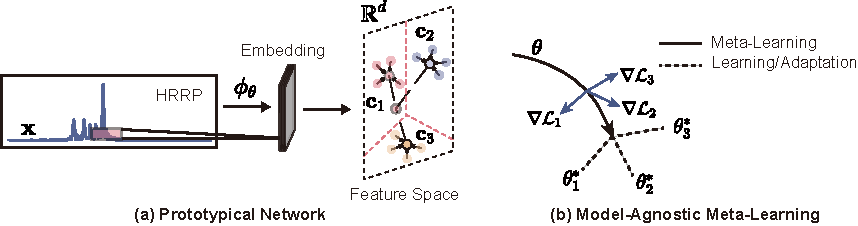
\includegraphics[width=\linewidth]{figures/proto_maml.pdf}
    % \fbox{图 2.2: ProtoNet工作原理示意图 (占位符)}
    \caption{ProtoNet工作原理示意图}
    \label{fig:protonet}
\end{figure}

基于优化的元学习方法,其目标是学习一个模型的初始参数 $\theta_0$(作为元参数 $\Phi$),使得该初始参数能通过在新任务 $\mathcal{T}_i$ 的支持集 $\mathcal{S}_i$ 上进行少量梯度下降更新,快速适应到对该任务最优的参数 $\theta_i'$。MAML\upcite{finn_model-agnostic_2017}是该方向的代表作。其元训练包含两个嵌套优化循环。内循环是任务适应:对于任务 $\mathcal{T}_i=(\mathcal{S}_i, \mathcal{Q}_i)$,从当前元参数 $\theta$ 出发,使用 $\mathcal{S}_i$ 计算损失 $\mathcal{L}_{\mathcal{S}_i}(\theta)$,并进行一步或 $U$ 步梯度下降更新得到任务特定参数 $\theta_i'$。例如,一步更新:
\begin{equation}
    \theta_i'(\theta) = \theta - \alpha \nabla_\theta \mathcal{L}_{\mathcal{S}_i}(\theta)
    \label{eq:maml_inner_update}
\end{equation}
其中 $\alpha$ 是内循环学习率。外循环是元优化:使用 $\mathcal{Q}_i$ 评估适应后的模型 $f_{\theta_i'}$,计算损失 $\mathcal{L}_{\mathcal{Q}_i}(\theta_i')$。元参数 $\theta$ 的更新基于所有任务的查询集损失梯度:
\begin{equation}
    \theta \leftarrow \theta - \beta \nabla_\theta \left( \sum_{\mathcal{T}_i \sim p(\mathcal{T})} \mathcal{L}_{\mathcal{Q}_i}(\theta_i'(\theta)) \right)
    \label{eq:maml_outer_update}
\end{equation}
其中 $\beta$ 是外循环学习率。计算元梯度 $\nabla_\theta \mathcal{L}_{\mathcal{Q}_i}(\theta_i'(\theta))$ 通常需要二阶导数,计算成本较高,存在一阶近似方法如FOMAML\upcite{yang_few-shot_2022}和Reptile\upcite{nichol_reptile_2018}以及简化方法ANIL\upcite{aniruddh_anil_2020}。MAML的核心是找到一个对任务损失变化敏感的初始化点。其优点是模型无关性。然而,MAML的训练可能不稳定,且对于HRRP的角度敏感性问题,仅仅几步梯度更新是否足以适应剧烈的特征变化也是一个疑问。

% --- 示意图占位符 ---
% \begin{figure}[h!]
%     \centering
%     \includegraphics[width=0.4\linewidth]{figures/maml.pdf}
%     % \fbox{图 2.3: MAML工作原理示意图 (占位符)}
%     \caption{MAML工作原理示意图}
%     \label{fig:maml}
% \end{figure}

元学习框架为解决小样本RATR问题提供了强大武器。通过元训练,模型有望学习到关于HRRP数据、类别关系及学习策略的元知识,从而在面对真实小样本场景时表现出更好的泛化性和适应能力。后续章节将深入探讨如何将元学习框架与针对性机制结合,以应对噪声、角度敏感性及语义信息利用不足等具体问题。

\section{本章小结}
\label{sec:theory_summary}
本章首先从物理层面深入剖析了HRRP的成像机理,推导了宽带雷达信号模型与HRRP的数学表达式,揭示了其与目标散射中心分布的关系及距离分辨率特性。通过引入噪声与杂波模型,形式化了低SNR对HRRP识别构成的第一个关键问题。进一步地,结合电磁散射理论和散射中心模型分析,阐明了HRRP对姿态角 $p(r; \theta, \phi)$ 的极端敏感性源于散射投影变化和相干干涉,并指出这是识别面临的第二个关键问题。这些分析为后续章节理解HRRP数据特性、应对噪声干扰与角度变化奠定了物理基础。

其次,本章回顾了基于深度学习的RATR框架,包括优化目标和典型模型。接着,对FSL问题进行了形式化定义,引入了S/Q Training范式,并从特征空间角度分析了小样本下特征判别性不足及语义信息 $s$ 缺失构成的第三个关键问题。最后,重点介绍了元学习框架及基于度量学习和基于优化这两大主流范式的数学原理。本章通过梳理相关基础理论并形式化关键问题,为后续章节针对性地提出基于元学习的解决方案提供了统一的数学语言和坚实的理论铺垫。